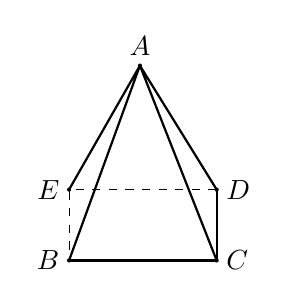
\begin{tikzpicture}[scale=.75,>=stealth]
\coordinate (B) at (0,0); \coordinate (C) at (2.5,0);
\coordinate (D) at (2.5,1.2); \coordinate (E) at (0,1.2);
\coordinate (A) at (1.2,3.3);
\draw[thick] (B)--(C)--(D); \draw[dashed] (D)--(E)--(B);
\draw[thick] (A)--(B) (A)--(C) (A)--(D) (A)--(E);
\draw[dashed] (A)--(D);
\fill (A) circle (1pt) node[above] {$A$};
\fill (B) circle (1pt) node[left] {$B$};
\fill (C) circle (1pt) node[right] {$C$};
\fill (D) circle (1pt) node[right] {$D$};
\fill (E) circle (1pt) node[left] {$E$};
\end{tikzpicture}
